\section{Definition}

\subsection{Project Overview}

My name is Fedor Smirnov and I am currently pursuing a Phd degree in Computer Science at the University of Erlangen-Nuremberg in Germany. Beside their research work, all phd students who work in our department also participate in teaching activities by giving exercise courses where the students work on problems that help them to understand and learn computer science topics necessary for their studies. Although preparing these courses takes quite some time and does not directly help me with my research work, I enjoy the teaching activities very much.

One thing that bothers me about the teaching organization is that all the people responsible for the teaching (the professors and the phd students) do not have any pedagogic background or education. Nevertheless, the phd students have to come up with exercises that can be used to effectively convey the topics addressed in the courses. I myself find it very hard to estimate how well an exercise that is organized in a certain way is suited to teach concepts to the students.

As my capstone project in the machine learning nanodegree, I would like to create a framework that can be used to evaluate the effectiveness of an exercise and (by altering the input) provide hints how altering the structure of the exercise (for example the number of steps, the number of problems that has to be practiced or the number of hints that the tutor should provide for specific steps) can improve its effectiveness. When I am talking about the effectiveness of an exercise, I mean that an exercise is effective if at the end of it, the students have learned to handle the underlying problem and would be able to solve the problem correctly without requiring any help if they encounter the problem again.

Following the recommendation of my reviewer of the capstone proposal, I will be concentrating on a subproblem of the framework, namely the clustering of the students onto different performance groups. 


\subsection{Related Work}
Searching for ways to provide more effective learning experiences for students who learn in classroom environments has been a popular research topic, especially after the publication of \cite{2sigma}. There, the authors present evidence that, depending on the learning environment, students of the same performance level can differ in their mastery of the taught subject by as much as two Sigma, i.e., two times the standard deviation.

Subjects where the classes can be taught via virtual tutoring programs are especially interesting for this area of research, as they offer an opportunity for a relatively easy acquisition and detailed analysis of huge amounts of data. The authors of \cite{machine_learning1} and \cite{machine_learning2} show how the data sets of these problems can be used to make the learning more effective (meaning that a skill can be mastered with a smaller number of exercises) and to optimize the schedule in order to prevent under- and over-practicing.

An experimental evaluation of each possible adjustment of the teaching process would be extremely time consuming. Consequently, a model for the prediction of the student performance is a key component of approaches for the optimization of teaching systems. This model takes a description of the students and the exercise and provides an estimation of the student performance, hereby enabling the implementation of the optimization loop illustrated in Fig.~\ref{fig_data_model}.

\begin{figure}
	\centering
	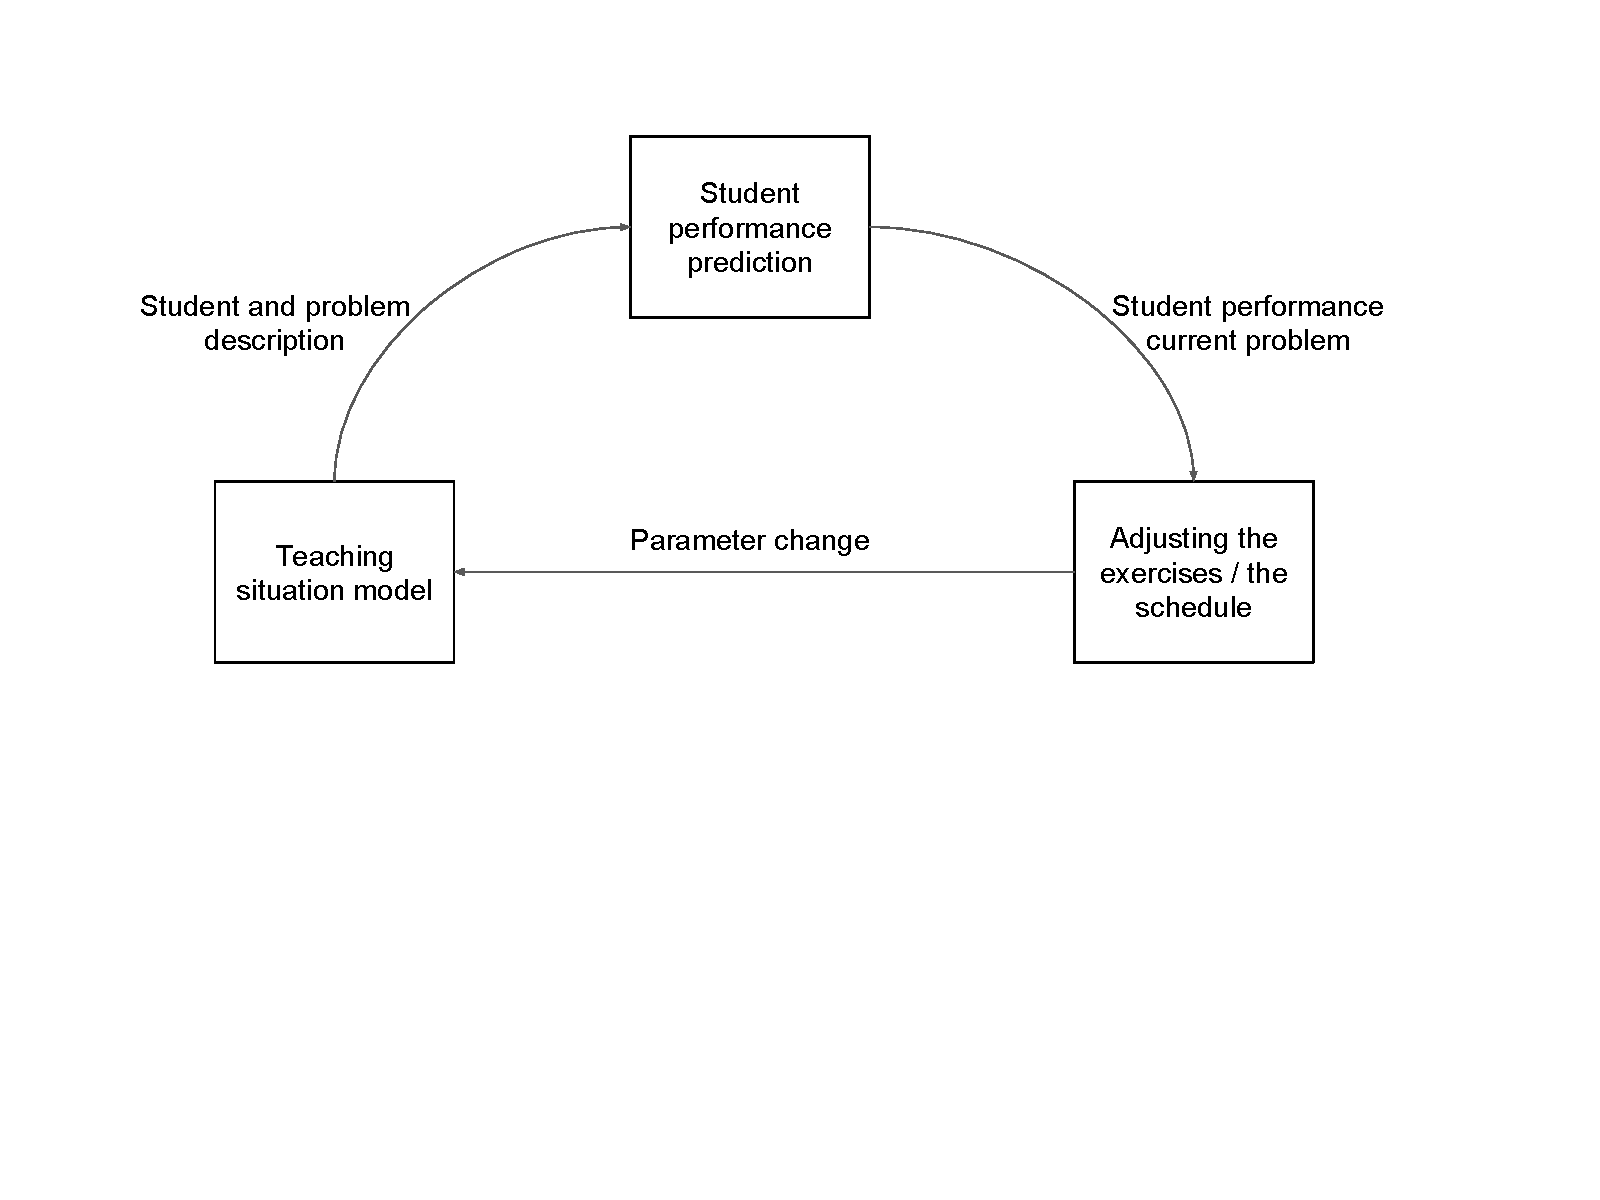
\includegraphics[width=\textwidth]{./img/data_model.pdf}
	\vspace{-3.5cm}
	\caption{A model for the prediction of the student performance can be used for an iterative optimization of the teaching situation.\label{fig_data_model}}
\end{figure}

Here, the effect of each change of the teaching situation, like using a different exercise structure or presenting the exercises in a different order, on the investigated objective function, like the general performance of the students or their learning rate, is estimated with the help of the performance prediction. The teaching situation can then be iteratively changed into the direction of an improving objective function.

As a basis for the student performance prediction, most state-of-the-art approaches rely on the so-called Learning Factors Analysis (LFA) model. There, the prediction of the student performance is done based on the following equation \cite{equation}:

\begin{equation}
	\log (\frac{P_{ijt}}{1 - P_{ijt}}) = \sum(\theta_i X_i) + \sum(\beta_j Y_j) + \sum (\gamma_j Y_j T_{jt})
\end{equation}

In this equation, the sum of the overall “smarts” (i.e., strength in the different skill fields) of the student ($\theta_i$), the “easiness” of a knowledge component (KC) and the amount of experience gained ($\gamma_j$) for each practice opportunity is used to calculate the probability that the $i$-th student will get a problem based on the $j$-th KC right when presented with the $t$-th opportunity to practice the KC. When applying this model, a key assumption is that the solution of each problem can be seen as an opportunity for the application of one or multiple KCs. A KC is hereby a generalization of all pieces of information that can be used for the accomplishment of a task, like concepts or skills. Identifying the KCs that the given problems are based on then becomes the main challenge for the creation of the student performance model.

Figure \ref{fig_kc_opt} illustrates the state-of-the-art approach that is used for the creation of a student performance model. 


\begin{figure}
	\centering
	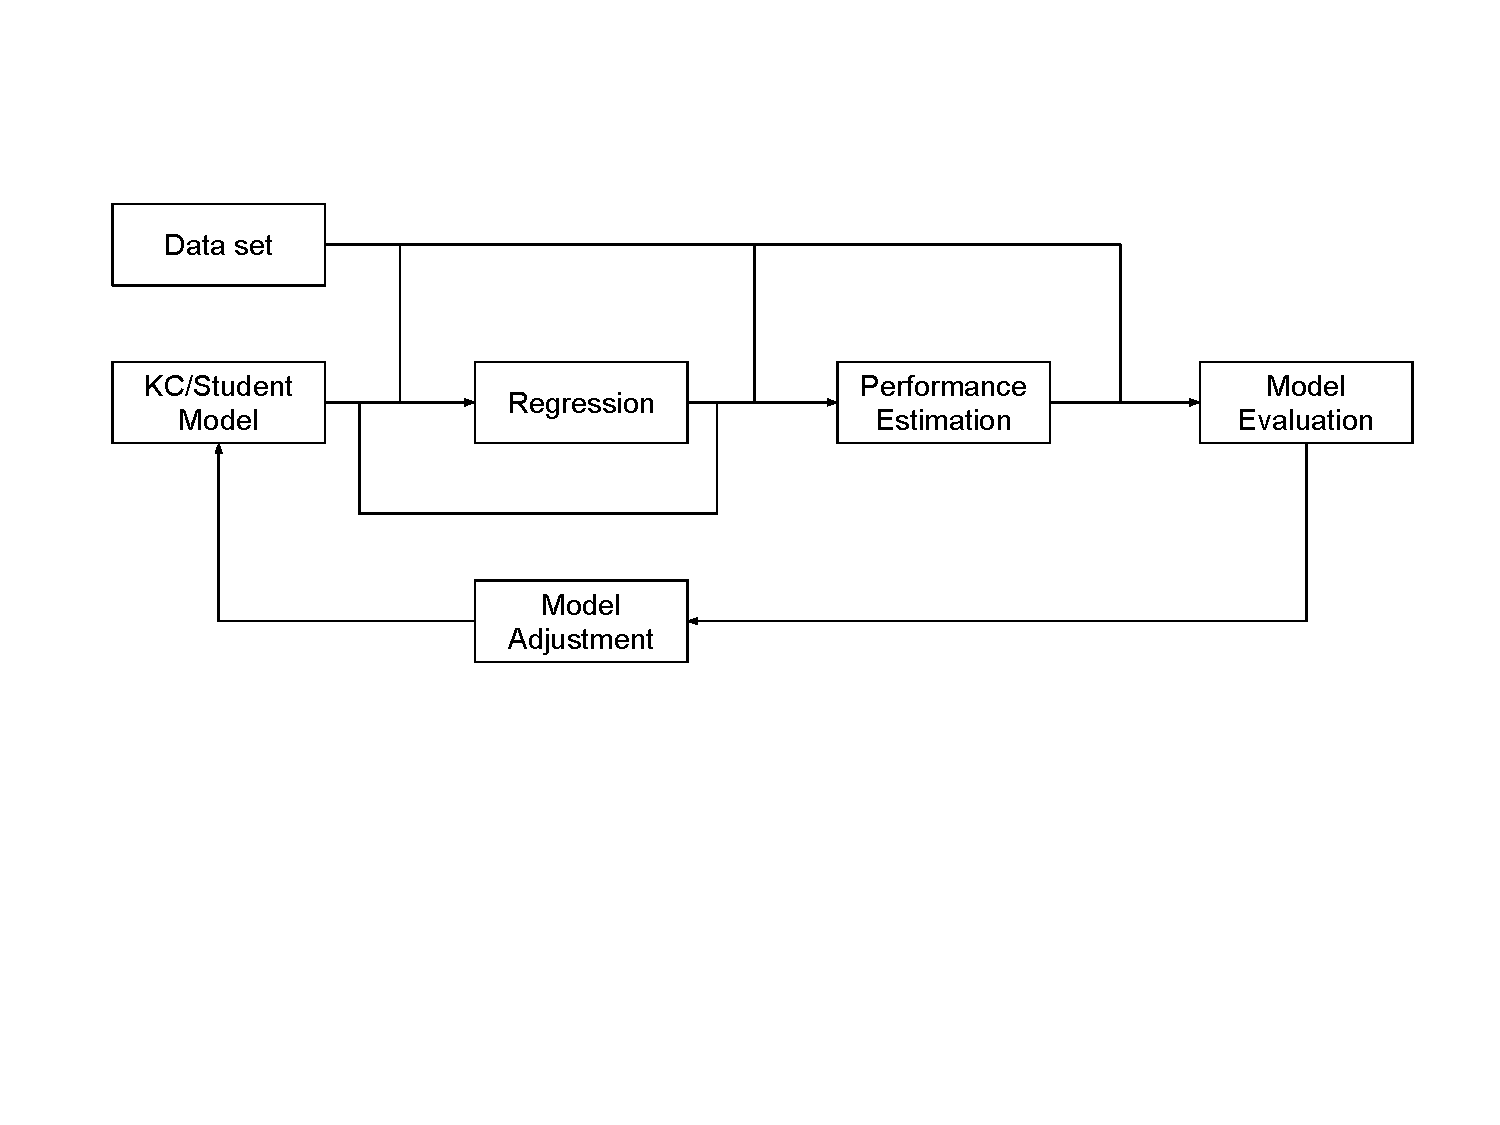
\includegraphics[width=\textwidth]{./img/kc_opt.pdf}
	\vspace{-3.5cm}
	\caption{Iterative optimization. In the first step, a regression model is used to fit the current KC model to the data by adjusting the weighting factors for the students’ smarts and the KCs’ easiness. This fitted model is then used for the estimation of the investigated objective like, e.g., the learning rate. The difference to the objective calculated using the actual data set (the error rate of the current KC/student model) is then iteratively minimized by adjusting the KC/student model.   
		\label{fig_kc_opt}}
\end{figure}

A KC/student that provides a small error relatively to the real data set enables a precise estimation of the student performance and can, consequently, be used for the estimation of the effect that certain changes of the teaching situation will have on the student performance.


\subsection{Problem Statement}\label{la_problem_statement}
The framework that I want to create will take a description of the exercise that is being evaluated (number of steps, skill level of the students in the class, number and/or kind of knowledge components necessary to solve the problem) and classify the exercise as effective or not effective. If an exercise is effective, the students who have finished it (in the way specified by the input, for example through hints from the tutor) will be able to solve this problem correctly and without help when they encounter it the next time. Otherwise the exercise is considered to be ineffective.

The framework that I want to create has two key differences to the state-of-the-art approach presented in the last section. On the one hand, I intend to apply a model trained with certain data (solving algebra problems) for the performance evaluation of problems from an entirely different field (computer science). On the other hand, I want this framework to be usable for tutors not having knowledge about the KC- or student models. The framework consequently has to work with inputs that can be intuitively provided by the tutors, rather than the features found in the data sets used for the training of the framework’s predictions models.

The overall vision of the framework is depicted in Fig.~\ref{fig_vision}:

\begin{figure}
	\centering
	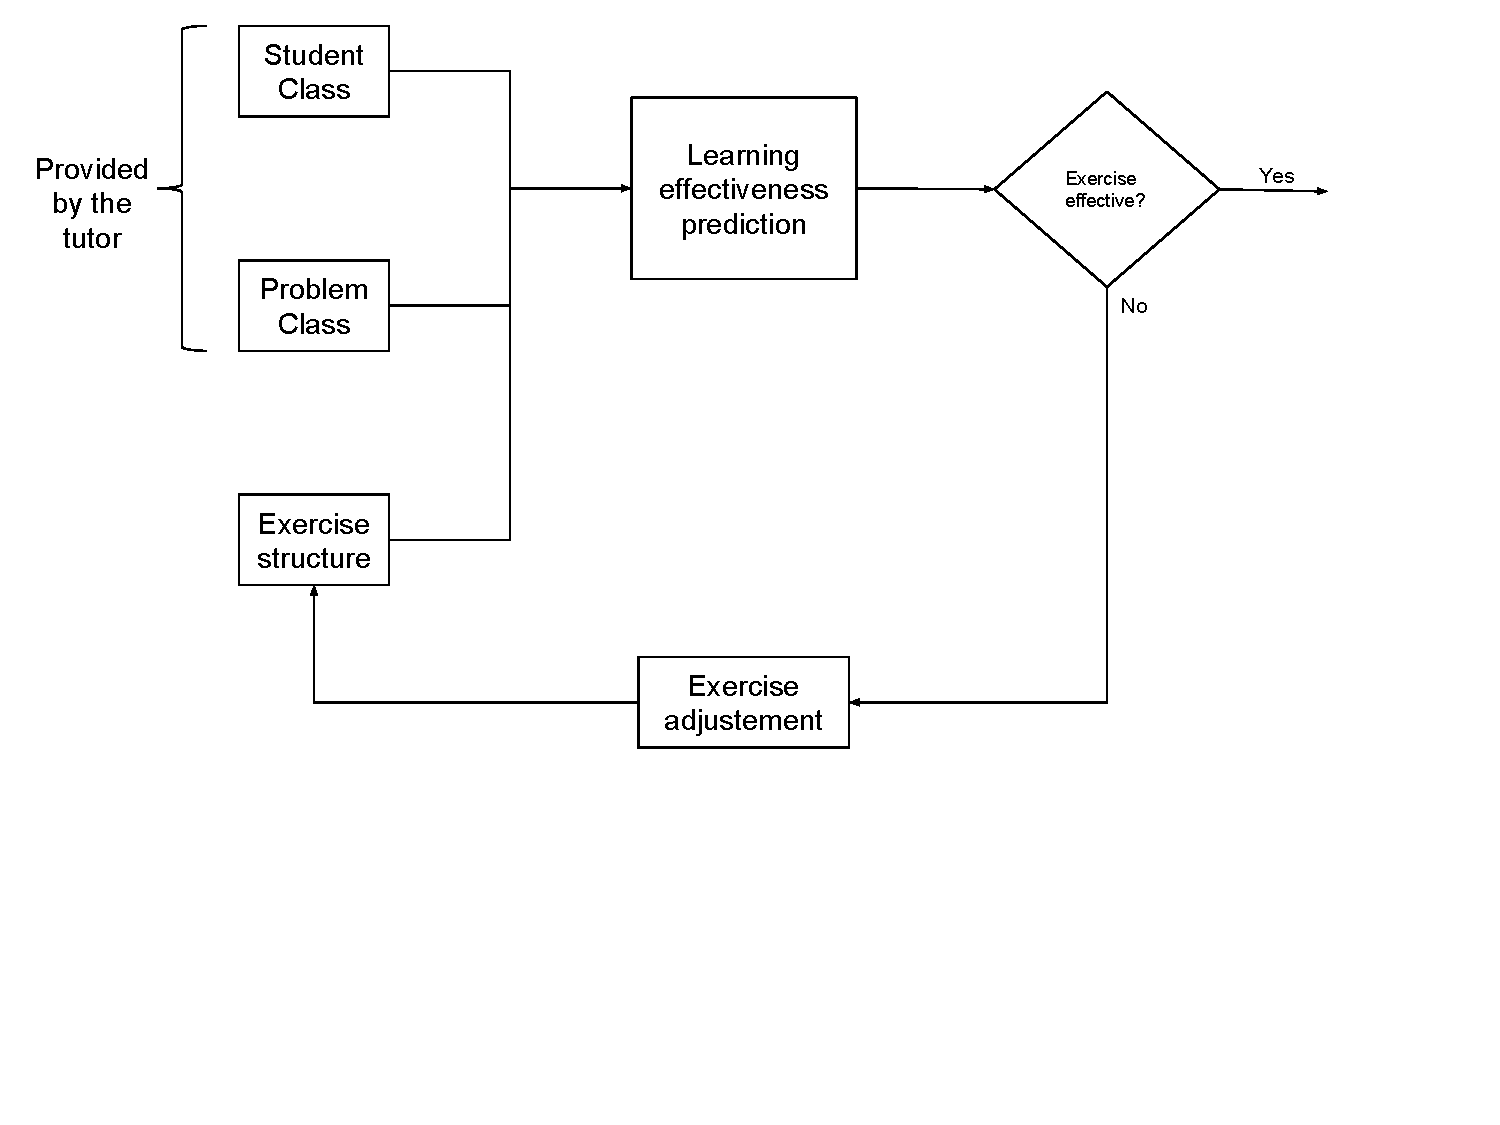
\includegraphics[width=\textwidth]{./img/vision.pdf}
	\vspace{-3.5cm}
	\caption{The tutor provides his assessment of the difficulty of the problem and the skill level of the students in the course along with the current structure of the exercise. The framework then predicts whether the exercise is effective in the current form or whether the tutor has to adjust its structure.\label{fig_vision}}
\end{figure}

\begin{enumerate}
	\item The tutor provides abstract, subjective descriptions of the problem that is treated in the evaluated exercise and of the students that this exercise is intended for.
	\item In addition to this, the tutor describes the current structure of the exercise that will be used to teach the students to handle the problem at hand.
	\item The trained prediction model (the “Learning effectiveness prediction” block in Fig.~\ref{fig_vision}) takes these inputs and provides a prediction about the effectiveness of the exercise which classifies the structure of the exercise as effective or not. If the exercise is classified as ineffective, the tutor adjusts its structure and performs the next evaluation iteration.
\end{enumerate}

As detailed in the capstone proposal, the problem that is addressed in this project can be divided into three subproblems. 

Training the effectiveness prediction is obviously an important step during the framework creation. However, the data set that is used throughout this project describes the learning process of students that are using an on-line framework to learn algebra related problems. The situation in which the data set was gathered differs from the situation addressed in this project in two important aspects: \textbf{a)} the problems that the students were solving come from a different domain and  \textbf{b)} the data set contains information that will not be accessible for the tutors of a university class, like, e.g., the exact time that was needed for solving the problem steps. Consequently, the data set can not be used for the training of the prediction model without a preprocessing step. During this preprocessing, the detailed data set entries describing the students and the problems have to be mapped onto subjective categories that can be intuitively used by the tutors. A schematic of the three subproblems is given in Fig.~\ref{fig_sub_problems}.

\begin{figure}
	\centering
	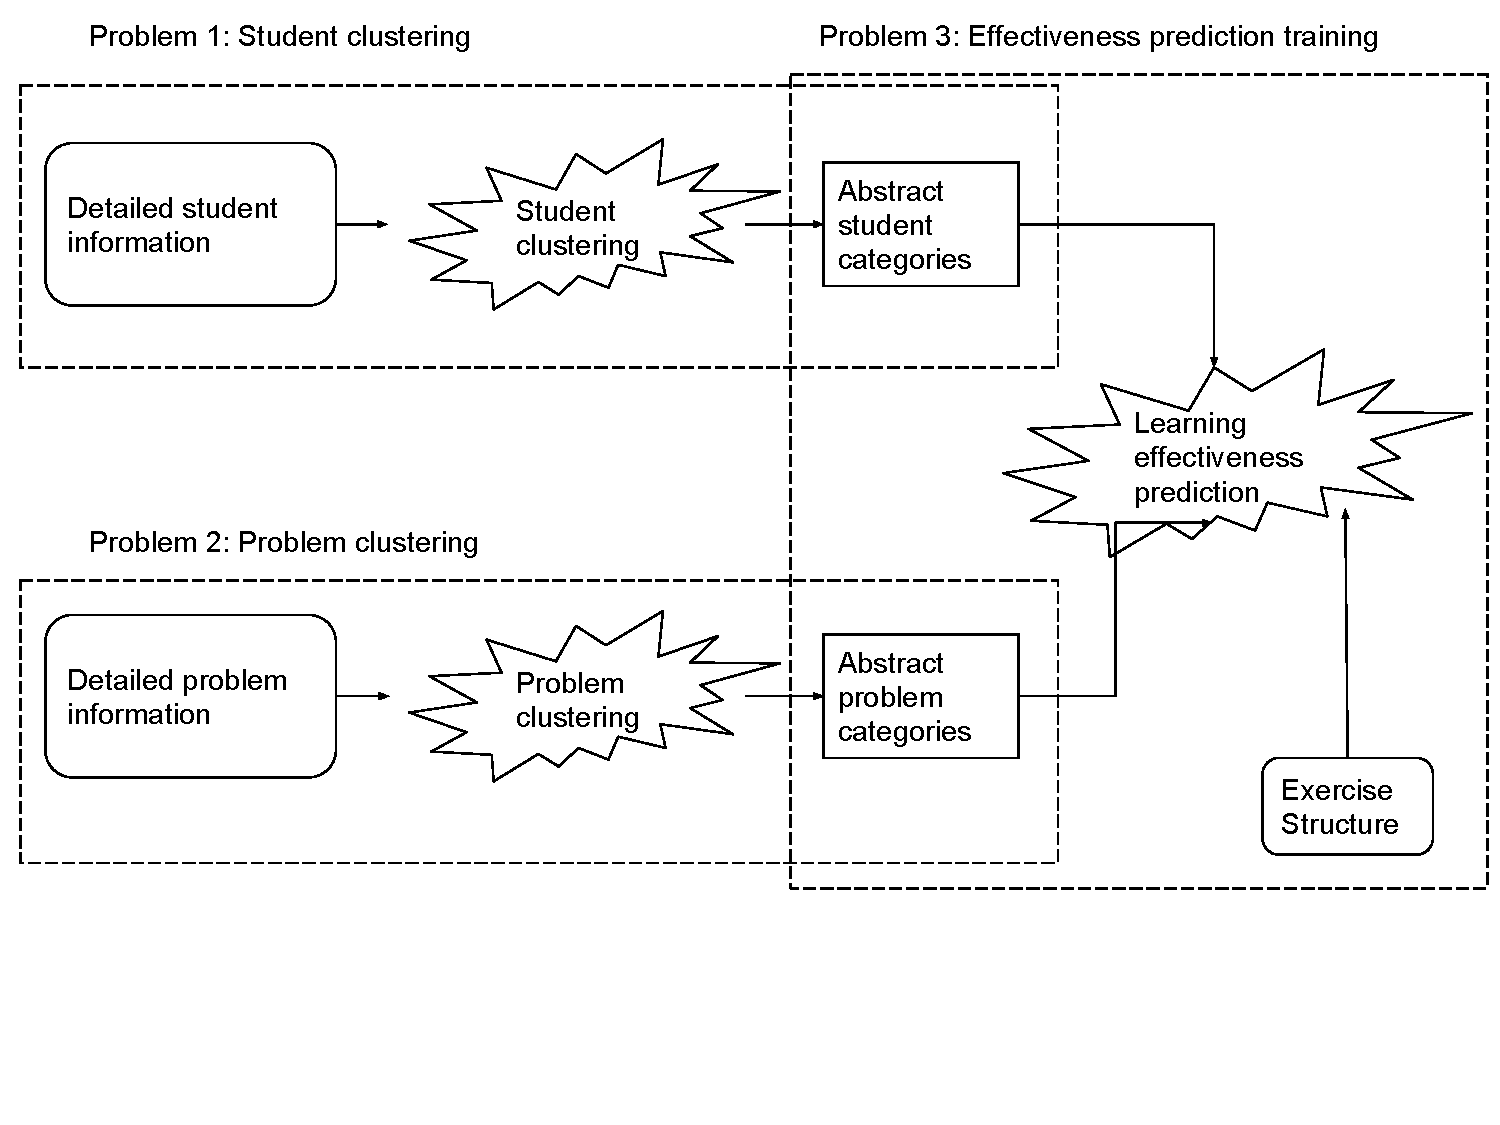
\includegraphics[width=\textwidth]{./img/subProblems.pdf}
	\caption{The overall problem can be divided into three subproblems \label{fig_sub_problems}}
\end{figure}

Following the recommendation of the reviewer of my capstone proposal, I would like to concentrate on one of the subproblems during the capstone project that I am doing in the scope of the Nanodegree and complete the other problems as a hobby project. The problem I would like to concentrate on is the clustering of the students on the abstract student categories (Problem 1 in Fig.~\ref{fig_sub_problems}).

\paragraph{Problem Description:}

The goal of the student clustering is a mapping, where the attributes from the KDD cup data set (consisting of measurements such as the time for the problem solutions) can be mapped onto more abstract student categories that a tutor would use to describe the skill level of students. In a way, the goal of the student clustering is the creation of a model that allows to transform the measurable attributes found in the KDD data set into the hidden features describing the skill levels of the students.

\paragraph{Problem Approach/Task Outline:}

To create a model capable of clustering the students onto categories describing the students’ skill level, the following tasks have to be carried out:

\begin{enumerate}
	\item Data analysis / Preprocessing
	\item Feature engineering
	\item Clustering
	\item Evaluation
\end{enumerate}

\begin{description}
	\item[Data Analysis] The first step of the student clustering is an analysis of the data provided in the KDD data set. At the very start, I hereby intend to check the data for completeness to rule out the possibility that certain attributes are only present in a small subset of the data, making them useless for the clustering. In the next step, I will gather information describing the overall set (for example the number of individual students or the number of exercises processed by each student). In the final step of the data analysis, I then will check each feature in the KDD set and decide \textbf{a)} whether it is, in my opinion, likely to be relevant to describe the student’s skill level and \textbf{b)} whether this feature is accessible for a tutor trying to assess the skill level of his/her students or not (e.g., the exact time the students need for the exercises that were carried out in the past will not be known to the tutor designing the exercise. On the other hand, the information whether or not the students have seen a  similar problem in the past is something that the tutor is likely to know). This distinction is important, as features that are not accessible for the tutor can not be part of the input provided for subproblem 3 and consequently, have to be transformed onto abstract categories while the accessible features may be directly used by the tutor as input for the learning effectiveness prediction.
	
	\item[Feature Engineering] The goal of the feature engineering step is a transformation of the features of the KDD data set onto the hidden feature describing the skill level of the students. On the one hand, this step will reduce the number of features used as the input for the clustering algorithm, hereby hopefully preventing overfitting. On the other hand, it will create new features describing the students and give me a feeling for the overall qualities that determine the cluster the students are associated with. At this point, I intend to apply PCA and experiment with different numbers of components. The overall goal of the student clustering is to be able to work with categories that are understandable for the tutors. It is consequently very important that the new features created by the feature engineering step can be interpreted with respect to a certain student quality.
	
	\item[Clustering] The goal of the clustering step is to take in the features provided by the feature transformation and use them to cluster the students. The clustering does not necessarily have to be done according to the skill level, but the result has to be interpretable so that the tutors have the possibility to determine the group their students can be assigned to. In this step, I intend to try different clustering algorithms and different sets of features in order and choose which combination delivers the best result. The results hereby will be evaluated based on the confidence with which the students are assigned to different groups and on how well the results can be interpreted and explained by an observable quality of the students.
	
	\item[Evaluation] As the objective of the clustering is to assign students to a skill group, I think a good way to evaluate the results is to examine whether the membership of a student to a skill group correlates with their relative strength within the student group, i.e., their position in a list where the students are ordered based on their relative correctness. 
\end{description}

\subsection{Metrics}

As described in section \ref{la_problem_statement}, I will evaluate the results of the student clustering by comparing them to a list where the students are ordered based on the average correctness that they achieved in the problem steps they carried out. Basically, both the trained clustering algorithm and the correctness list will work similarly to a classifier, in that it will assign a label to a student indicating the performance group that the student is in. For the case of 2 performance groups, the correctness list and the clustering processing a student $s$ can be written as $L(s)$ and $C(s)$, respectively. Hereby, the result of the correctness list will be 1 if the student has had a high correctness ($L(s) = 1$) and be 0 otherwise ($L(s) = 0$). Similarly, the result of the clustering operation will indicate whether the student is predicted to be part of the very skilled cluster ($C(s) = 1$) or not ($C(s)=0$). 

I expect that the students that can be found in the same clusters will have a similar position on the correctness list. If the clustering results differ from the correctness list in a significant way, the reason for this difference has to be investigated.

Although I do expect a certain degree of correlation between the clustering results and the correctness list, I think that a certain degree of difference is also desirable. Otherwise, no clustering would be needed and we could simply use the average exercise correctness to classify the students.

Hereby, the correlation between the clustering result and the correctness list can be measured by metrics similar to those used to evaluate the result of classification algorithms. I intend to measure the rate of true positives $T_p$, true negatives $T_n$, false positives $F_p$, and false negatives $F_n$. For a student set $S$, these metrics are described by the following equations:

\begin{equation}
	T_p = \frac{|L(S)=1 \wedge C(S)=1|}{|S|}
\end{equation}

\begin{equation}
	T_n = \frac{|L(S)=0 \wedge C(S)=0|}{|S|}
\end{equation}

\begin{equation}
	A = T_p + T_n
\end{equation}

\begin{equation}
	F_p = \frac{|L(S)=0 \wedge C(S)=1|}{|S|}
\end{equation}

\begin{equation}
	F_n = \frac{|L(S)=1 \wedge C(S)=0|}{|S|}
\end{equation}

$T_p$, hence, describes the fraction of the students that are predicted to be very skilled and at the same time have a high average correctness. $T_n$ is the fraction of students that are predicted to be less able and at the same time have a low average correctness. $A$ describes something similar to the accuracy score, i.e., the fraction of students where the clustering prediction matches the students' position in the correctness list. $F_p$ describes the probability for a student with a low average correctness to be predicted to be skilled, while $F_n$ describes the opposite case where a student with a high average correctness is predicted to be less able.

For a promising clustering, I would expect a high (higher than 50\%), yet not a perfect $A$-value.
 